% ALGUNOS PAQUETES REQUERIDOS (EN UBUNTU): %
% ========================================
% %
% texlive-latex-base %
% texlive-latex-recommended %
% texlive-fonts-recommended %
% texlive-latex-extra %
% texlive-lang-spanish (en ubuntu 13.10) %
% ******************************************************** %

\documentclass[a4paper]{article}
\usepackage[spanish]{babel}
\usepackage[utf8]{inputenc}
\usepackage{fancyhdr}
\usepackage[pdftex]{graphicx}
\usepackage{sidecap}
\usepackage{caption}
\usepackage{subcaption}
\usepackage{booktabs}
\usepackage{makeidx}
\usepackage{float}
\usepackage{amsmath, amsthm, amssymb}
\usepackage{amsfonts}
\usepackage{sectsty}
\usepackage{wrapfig}
\usepackage{listings}
\usepackage{enumitem}
\usepackage{hyperref}
\usepackage{listings}
\usepackage{listingsutf8}
\usepackage{enumitem}

% Para ver los marcos
% \usepackage{showframe}

\newcommand{\ord}{\ensuremath{\operatorname{O}}}
\newcommand{\nat}{\ensuremath{\mathbb{N}}}
\renewcommand{\thesubsubsection}{\thesubsection.\alph{subsubsection}}

% Lemas, definiciones, etc.
\theoremstyle{remark}
\newtheorem*{obs}{Observación}
\newtheorem*{nota}{Notación}
\newtheorem*{cor}{Corolario}
\theoremstyle{definition}
\newtheorem*{defi}{Definición}
\theoremstyle{plain}
\newtheorem{teo}{Teorema}
\newtheorem{lema}{Lema}
\newtheorem{prop}{Propiedad}

\usepackage{fancyhdr}
% \pagestyle{fancy}
%\renewcommand{\chaptermark}[1]{\markboth{#1}{}}
\renewcommand{\sectionmark}[1]{\markright{\thesection\ - #1}}
\fancyhf{}
% \fancyhead[LO]{Sección \rightmark} % \thesection\

% \fancyfoot[RO]{\thepage}
\renewcommand{\headrulewidth}{0.5pt}
\renewcommand{\footrulewidth}{0.5pt}
%\setlength{\hoffset}{-0.8in}
\setlength{\textwidth}{16cm}
\setlength{\hoffset}{-1.1cm}
\setlength{\headsep}{0.5cm}
\setlength{\textheight}{25cm}
\setlength{\voffset}{-0.7in}
\setlength{\headwidth}{\textwidth}
\setlength{\headheight}{13.1pt}
\renewcommand{\baselinestretch}{1.1} % line spacing


\begin{document}

\title{Teoría de las comunicaciones}
\author{Manuel Mena}
\maketitle

\tableofcontents

\newpage
\section{Práctica 1}

\subsection{}

\subsubsection{}
$I(s) = -log_2(P(s))$

\begin{tabular}{rl}
$H(S)$ & $= \sum_{s \in S}(P(s) I(s))$ \\
& $= (P(s_0) I(s_0)) + (P(s_1) I(s_1))$ \\
& $= (p_0 (-log_2(p_0))) + (1 - p_0) (-log_2(1 - p_0)))$ \\
& $= -p_0 log_2(p_0) - log_2(1 - p_0) + p_0 log_2(1 - p_0)$ \\
& $= p_0(log_2(1 - p_0) -log_2(p_0)) - log_2(1 - p_0)$ \\
& $= p_0 * log_2(\frac{1 - p_0}{p_0}) - log_2(1 - p_0)$ \\
\end{tabular}

\subsubsection{}

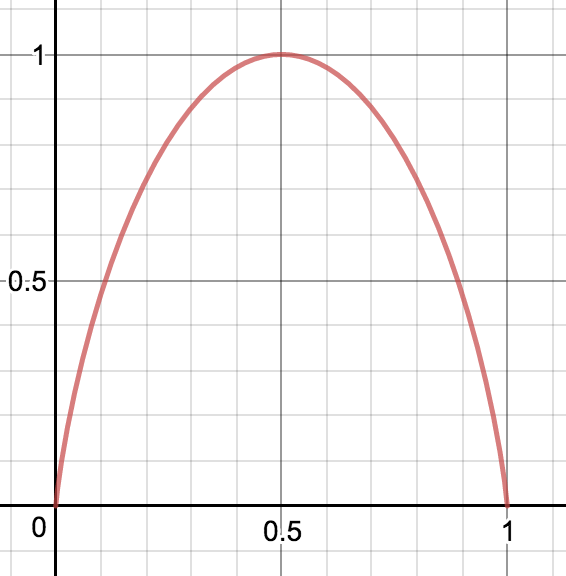
\includegraphics{imagenes/1_1_b.png}

\subsection{}

\subsubsection{}
El tercero

\subsubsection{}
El segundo y el tercero

\subsubsection{}
\begin{tabular}{rl}
$H(S)$ & $= \sum_{s \in S}(P(s) I(s))$ \\
& $= 0.4 (-log_2(0.4)) + 0.3 (-log_2(0.3)) + 0.2 (-log_2(0.2)) + 0.1 (-log_2(0.1))$ \\
& $= 1.84643934467$ \\
\end{tabular}

\begin{tabular}{rl}
$L(segundo)$ & $= \sum_{s \in S}(P(s)|C(s)|)$ \\
& $= 0.4 * 1 + 0.3 * 2 + 0.2 * 3 + 0.1 * 3$ \\
& $= 1.9$ \\
\end{tabular}

\begin{tabular}{rl}
$L(tercero)$ & $= \sum_{s \in S}(P(s)|C(s)|)$ \\
& $= 0.4 * 1 + 0.3 * 2 + 0.2 * 3 + 0.1 * 4$ \\
& $= 2$ \\
\end{tabular}

Eficiencia segundo: 0,9718101814

Eficiencia tercero: 0,9232196723

El segundo es más eficiente.

\subsubsection{}
No, puesto que $H(S) \leq L(C)$ en ambos casos.

\subsection{}

\subsubsection{}
\begin{tabular}{rl}
$H(S)$ & $= \sum_{s \in S}(P(s) I(s))$ \\
& $= 0.5 (-log_2(0.5)) + 0.5 (-log_2(0.5))$ \\
& $= 1$ \\
\end{tabular}

\begin{tabular}{rl}
$L(C)$ & $= \sum_{s \in S}(P(s) |C(s)|)$ \\
& $= 0.5 * 1 + 0.5 * 1$ \\
& $= 1$ \\
\end{tabular}

\subsubsection{}
\begin{tabular}{rl}
$H(S)$ & $= \sum_{s \in S}(P(s) I(s))$ \\
& $= 0.25 (-log_2(0.25)) + 0.25 (-log_2(0.25)) + 0.25 (-log_2(0.25)) + 0.25 (-log_2(0.25))$ \\
& $= 2$ \\
\end{tabular}

\begin{tabular}{rl}
$L(C)$ & $= \sum_{s \in S}(P(s) |C(s)|)$ \\
& $= 0.25 * 2 + 0.25 * 2 + 0.25 * 2 + 0.25 * 2$ \\
& $= 2$ \\
\end{tabular}

\subsubsection{}
\begin{tabular}{rl}
$H(S)$ & $= \sum_{s \in S}(P(s) I(s))$ \\
& $= \frac{1}{6} (-log_2(\frac{1}{6})) + \frac{1}{6} (-log_2(\frac{1}{6})) + \frac{1}{6} (-log_2(\frac{1}{6})) + \frac{1}{6} (-log_2(\frac{1}{6})) + \frac{1}{6} (-log_2(\frac{1}{6})) + \frac{1}{6} (-log_2(\frac{1}{6}))$ \\
& $= 2.58496250072$ \\
\end{tabular}

\begin{tabular}{rl}
$L(C)$ & $= \sum_{s \in S}(P(s) |C(s)|)$ \\
& $= \frac{1}{6} (-log_2(\frac{1}{6})) + \frac{1}{6} (-log_2(\frac{1}{6})) + \frac{1}{6} (-log_2(\frac{1}{6})) + \frac{1}{6} (-log_2(\frac{1}{6})) + \frac{1}{6} (-log_2(\frac{1}{6})) + \frac{1}{6} (-log_2(\frac{1}{6}))$ \\
& $= 2.58496250072$ \\
\end{tabular}

\subsubsection{}
\begin{tabular}{rl}
$H(S)$ & $= \sum_{s \in S}(P(s) I(s))$ \\
& $= 0.125 (-log_2(0.125)) * 8$ \\
& $= 3$ \\
\end{tabular}

\subsubsection{}
\begin{tabular}{rl}
$H(S)$ & $= \sum_{s \in S}(P(s) I(s))$ \\
& $= 0.1 (-log_2(0.1)) * 10$ \\
& $= -log_2(0.1)$ \\
& $= log_2(10)$ \\
& $= 3.32192809489$ \\
\end{tabular}

\subsubsection{}
\begin{tabular}{rl}
$H(S)$ & $= \sum_{s \in S}(P(s) I(s))$ \\
& $= \frac{1}{n} (-log_2(\frac{1}{n})) * n$ \\
& $= -log_2(\frac{1}{n})$ \\
& $= log_2(n)$ \\
\end{tabular}

\subsection{}
Acá lo mas importante es notar que cada vez que la fuente $D$ toma un símbolo
es independiente de la anterior, entonces se puede definir
$P_D(s) = (P_D(A) * P_A(s) si s \in A sino P_D(B) * P_B(s))$, con $P_D(A)$ y
$P_D(B)$ la probabilidad de que $D$ saque un símbolo de $A$ y de $B$,
respectivamente. Entonces la solución sería:

\begin{enumerate}
\item $P_D(s) = 1/16$ si $s \in A$ sino $1/32$, no es equiprobable
\item $P_D(s) = 1/64$ si $s \in A$ sino $3/64$, no es equiprobable
\item $P_D(s) = 1/32$ si $s \in A$ sino $3/64$, no es equiprobable
\item $P_D(s) = 1/12$ si $s \in A$ sino $1/48$, no es equiprobable
\end{enumerate}

\subsection{}

\subsubsection{}
Como la fuente es equiprobable:

\begin{tabular}{rl}
$H(S) $ & $= log_2|S|$ \\
&$= log_2(10^{640*480})$ \\
&$= 640 * 480 * log_2(10)$ \\
\end{tabular}

\subsubsection{}
En esta fuente equiprobable, tenemos que $H(S) = log_2(n)$, no siendo $n$ una potencia de 2. Esto implica que no podemos pensar en recurrir a un código (óptimo) que asigne $log_2(n)$ bits por imagen, pues por supuesto estos valores deben ser números enteros. No obstante, la aproximación más cercana a este valor es tomar exactamente $\lceil log_2(n) \rceil$ bits por imagen. De esta forma podremos armar un código que sea unívocamente decodificable (cada imagen recibe una tira de bits distinta) y localmente óptimo, entendiendo por esto que todo otro código que mapee cada imagen a una tira de bits de igual largo debe necesariamente poseer una longitud media igual o mayor.
Como nota adicional, extrapolando los conceptos plasmados en la resolución de este ejercicio, es interesante pensar en si, efectivamente, dada una fuente equiprobable S' de m símbolos, y dado un código C que actúe sobre S' definiendo para cada símbolo una codificación de largo $\lceil log_2(m) \rceil$ bits, se tiene que C es óptimo. Cuando m es potencia de 2, la respuesta es afirmativa (¿por qué?). En cualquier otro caso, y quizás yendo a contramano de la intuición, la respuesta es que no. Como ejemplo sencillo, considerar el caso en el que $m = 3$. Como $\lceil log_2(m) \rceil = 2$, tenemos que $L(C) = 2$. Sin embargo, podemos proponer un código alternativo C' que asigne un 0 a un símbolo, un 10 a otro y un 11 al restante. Es claro que C' es instantáneo, y además se ve claramente que $L(C') < 2 = L(C)$

\subsubsection{}
Para responder este ítem, hay que usar el teorema de Shannon: $C = B * log_2(1 + SNR)$. Primero, la relación señal-ruido hay que pasarla de decibeles a veces: $SNR = 10^{30/10} = 1000$. Luego, como se necesitan 30 imágenes por segundo, la capacidad de canal debe ser mayor o igual que $\lceil 640 * 480 * log_2(10) * 30 \rceil$ bps. Entonces, $B = (\lceil 640 * 480 * log_2(10) \rceil * 30)/ log_2(1001)$ Hz.

\subsection{}
Para calcular la capacidad de volumen, necesitamos $Delay$ y $V_{tx}$. Primero calculamos la Capacidad de Transmisión de Shannon para obtener la $V_{tx}$ (dejamos la resolución para el inciso b):

\begin{tabular}{rl}
$C$ & $= B * log_2(1 + SNR[dB])$ \\
& $= 400kHz * log_2(1 + 10[dB])$ \\
& $= 400kHz * log_2(1 + 10[veces]) \implies V_{tx} \leq 1383,7Kbps$ \\
\end{tabular}

Ahora Delay:

\begin{tabular}{rl}
$Delay$ & $= T_{prop} + T_{tx}$ \\
& $= \frac{D}{V_{prop}} + \frac{|Unidad de Datos|}{V_{tx}}$ \\
& $= \frac{100km}{200000km/s} + \frac{1bit}{1383Kbps} = 0,0005seg = 0,5ms$ \\
\end{tabular}

Finalmente:

$C_{vol} = Delay * V_{tx} = 691bits$

\subsection{}
$C_{max} = 100$Mbps \\
$V_{prop} = 300000$ km/s \\

\begin{tabular}{rl}
$Delay$ & $= T_{tx} + T_{prop}$ \\
$Delay$ & $= \frac{|datos|}{V_{tx}} + \frac{D}{V_{prop}}$ \\
$Delay$ & $= \frac{30Mb}{100Mbps} + \frac{D}{300000km/s}$ \\
$0.04s$ & $\geq \frac{30Mb}{100Mbps} + \frac{D}{300000km/s}$ \\
$0.04s - \frac{30Mb}{100Mbps}$ & $\geq \frac{D}{300000km/s}$ \\
$0.04s - 0.3$s & $\geq \frac{D}{300000km/s}$ \\
$(- 0.26)s * 300000km/s$ & $\geq D$ \\
$-78000km/s$ & $\geq D$ \\
\end{tabular}

No pueden existir distancias negativas. Siendo la velocidad de transmicion de 100 Mpbs, no pueden enviarse 30 Mb en menos de 0.3 s.

\subsection{}
\subsubsection{}
\begin{tabular}{rl}
$Delay$ & $= T_{prop} + T_{tx}$ \\
& $= \frac{D}{V_{prop}} + \frac{|Unidad de Datos|}{V_{tx}}$ \\
& $= \frac{385000km}{300000km/s} + \frac{1bit}{100Mbps}$ \\
& $= 1.29s$
\end{tabular}

$RTT = Delay * 2 = 2.58s$

\subsubsection{}
\begin{tabular}{rl}
$C_{vol}$ & $= Delay * V_{tx}$ \\
& $= 2.58s * 100Mbps$ \\
& $= 258Mb$ \\
\end{tabular}

\subsubsection{}
\begin{tabular}{rl}
$T_{total}$ & $= Delay_{ida} + Delay_{vuelta}$ \\
& $= T_{prop} + T_{tx_{ida}} + T_{prop} + T_{tx_{vuelta}}$ \\
& $= \frac{D}{V_{prop}} + \frac{|Unidad de Datos|_ida}{V_{tx}} + \frac{D}{V_{prop}} + \frac{|Unidad de Datos|_vuelta}{V_{tx}}$ \\
& $= \frac{2D}{V_{prop}} + \frac{|Unidad de Datos|_ida + |Unidad de Datos|_vuelta}{V_{tx}}$ \\
& $= \frac{2 * 385000km}{300000km/s} + \frac{2Kb + 25Mb}{100Mbps}$ \\
& $= 2.57s + \frac{2Kb + 25000Kb}{100000Kbps}$ \\
& $= 2.57s + \frac{25002Kb}{100000Kbps}$ \\
& $= 2.57s + 0.25s$ \\
& $= 2.82s$ \\
\end{tabular}


\newpage
\section{}

\subsection{}

\subsubsection{}
\begin{tabular}{rl}
$C_{vl}$ & $= Delay * V_{tx}$ \\
& $= 1.25s * 1Mbps$ \\
& $= 1.25Mb$ \\
\end{tabular}

\subsubsection{}
Entran $\frac{1.25Mb}{1Kb} = \frac{1250Kb}{1Kb} = 1250$ Frames

\subsection{}

\subsubsection{}
$Eframe = \frac{largo de los datos}{largo de los datos} = 1$

\subsubsection{}
$Eframe = \frac{largo de los datos}{largo de los datos + 16}$

\subsubsection{}
$Eframe = \frac{largo de los datos}{largo de los datos + 8 + bits incorporados debido al stuffing}$

\subsection{}

\subsubsection{}
Para el primer caso podríamos definir un frame para el emisor y otro para el receptor de la siguiente forma:

Emisor: \#SEQ(1bit); Datos; Checksum

Receptor: \#ACK(1bit); Checksum

\subsubsection{}
Para el segundo caso, al haber Piggybacking todos los frames pueden llegar a tener que cumplir simultáneamente los roles de emisión y recepción. Entonces proponemos un único frame como el siguiente:

\#SEQ; \#ACK; Datos; Checksum

\subsubsection{}
Para el último caso, a diferencia del punto anterior tenemos reconocimento selectivo. Para estos casos se recomienda, por un tema de eficiencia, que el frame receptor reconozca los frames tanto acumulativa como individualmente. Entonces nos quedarían dos frames como los siguientes:

Emisor: \#SEQ; Datos; Checksum

Receptor: \#ACK; \#SACK; Checksum


\setcounter{subsection}{4}
\subsection{}

\subsubsection{}
\begin{tabular}{rl}
$SWS$ & $= \frac{V_{tx} * RTT}{|Frame|}$ \\
& $= \frac{1Mbps * 2 * 0.25s}{2Kb}$ \\
& $= \frac{500Kb}{2Kb}$ \\
& $= 250$ \\
\end{tabular}

$RWS = 1$

\subsubsection{}
\begin{tabular}{rl}
$\#frames \geq SWS + RWS$ & $= \frac{V_{tx} * RTT}{|Frame|}$ \\
& $= \frac{1Mbps * 2 * 0.25s}{2Kb} + 1$ \\
& $= \frac{500Kb}{2Kb} + 1$ \\
& $= 251$ \\ \\

$\#frames$ & $\geq 251$ \\
\end{tabular}

Por lo tanto se necesitan $\lceil log_2(251) \rceil = 8$ bits.

\subsubsection{}
Frame: \#SEQ (8 bits); Datos (1976 bits) CRC (16 bits) (2Kb total)

$20Mb$ de datos $= \lceil \frac{20000000bits}{1976bits} \rceil$ frames $= 10.122$ frames

\begin{tabular}{rl}
$Delay(10122 Frames)$ & $= Delay(10122 * 2Kb)$ \\
& $= Delay(20122Kb)$ \\
& $= T_{tx}(20122Kb) + T_{prop}$ \\
& $= \frac{20122Kb}{V_{tx}} + 0.25s$ \\
& $= \frac{20122Kb}{1Mbps} + 0.25s$ \\
& $= 20.122s + 0.25s$ \\
& $= 20.372s$ \\
\end{tabular}

A esto se le agrega el envío de el último frame

\subsection{}

\subsubsection{}
$E_{frame} = \frac{largo de los datos}{largo total del frame} $

\subsection{}
$E_{proto} = \frac{T_{tx}(SWS)}{RTT}$

\newpage
\section{}

\subsection{}

\subsubsection{}
$t_{min} = 2 * Delay_{max} = 2 * 25.6 \mu s = 51.2 \mu s$

\subsubsection{}
$V_{tx} = 10 Mbps$

Regla de 3 simple. En un segundo transmito 10 Mb, en $51.2 \mu s$ transmito

$51.2 \mu s * 10Mbps = 51.2 \mu s * 10bp \mu s = 512bits = 64B$

\subsubsection{}
Se rellena con padding. Hay dos opciones para luego descartar el padding:

\begin{itemize}
\item En el header: en lugar de usar el campo type para multiplexar se usa como length tamaño y se usa LLC como multiplexador para la capa de red.
\item Se encarga la capa superior (por ejemplo IP length).
\end{itemize}

\subsubsection{}
Ambos sensan el medio en los respectivos momentos temporales e identifican que el medio está siendo utilizado. Ergo, esperan (1-persistente) hasta que el medio esté libre y luego transmiten. Ambos encontrarán el medio libre en momentos muy cercanos (la diferencia está dada por la distancia entre H2 y H3 con H1) y sus tramas colisionarán.

\subsubsection{}
H4 sensa el medio. Probablemente lo encuentre libre (por ejemplo si todavía no llega a sensar la información de la trama de H1 por estar a una distancia considerable), transmita y su trama colisione con la de H1.

\newpage
\section{}

\setcounter{subsection}{1}
\subsection{}
\subsubsection{}
Dependiendo de la version el formato del header es distinto, por lo que no saber que version es puede provocar no poder leer correctamente los campos.

\setcounter{subsubsection}{2}
\subsubsection{}
El tamaño máximo de un paquete IP es 65535 bytes. El campo lenght define este tamaño.

\subsection{}
\subsubsection{}
Tiene 3 interfaces: FastEthernet, Wireless0 Connection y Wirless1 Connection

\subsubsection{}
\begin{itemize}
\item Physical Address es la dirección MAC
\item IP Address es la direccion IP
\item Subnet Mask es la máscara de subred que se aplica
\item Default Gateway es el router por defecto
\end{itemize}

\subsection{}
\subsubsection{}
Es solo pasar los /N a XXX.XXX.XXX.XXX

/22 = 255.255.252.0

/23 = 255.255.254.0

/24 = 255.255.255.0

/25 = 255.255.255.127

\subsubsection{}
135.46.56.0/22 = 135.46. 0011 1000 .0 / 255.255.252.1111 1100 = 135.46.56.0

Capacidad máxima de hosts esta dada por /22, son todos las direcciones que podemos meter sobre los 10 digitos que la máscara anula. Osea $2^{10} = 1024$ hosts.

\subsubsection{}
\begin{tabular}{|c|c|c|}
\hline
& A & B \\ \hline
135.46.57.14 & Interface1 & descarta \\ \hline
135.46.63.10 & Interface0 & descarta \\ \hline
135.46.52.2 & 135.46.62.100 & descarta \\ \hline
208.70.188.15 & 135.46.62.100 & descarta \\ \hline
135.46.62.62 & Interface0 & descarta \\ \hline 
192.53.40.7 & 135.46.60.100 & Interface1 \\ \hline 
192.53.56.7 & 135.46.62.100 & descarta \\ \hline 
\end{tabular}

\subsection{}
PC1: 172.16.5.

\subsection{}
\subsubsection{}
Pueden direccionarse 256 - 2 hosts.

\subsubsection{}
2 subredes: 128 - 2 hosts.

4 subredes: 64 - 2 hosts.

8 subredes: 32 - 2 hosts.

\subsection{}
\subsubsection{}
Red A: 172.16.5.0/27 (32)

Red B: 172.16.5.32/29 (8) Dejo 8 porque se necesitan 1 host + 2 routers + 2 de broadcast y localhost

Red C: No puedo usar 15.16.5.40/27 (128) porque se solaparía con 17.16.5.64/22 que ya existe



\setcounter{section}{5}
\newpage
\section{Práctica 6}

\subsection{}
Un puerto es una interfaz a través de la cual se pueden enviar y recibir los
diferentes tipos de datos.

Si no se implementaran los puertos, entonces las aplicaciones de dos hosts
distintos se comunicarían de manera broadcast, ya que al enviar un dato se
estaría enviando a todo quien escuche en ese host. Teniendo puertos es posible
definir de donde recibir y hacia donde enviar.

UDP es mas rápido ya que hace menos chequeos pero es menos seguro y no es
confiable. Es útil en caso de una aplicación de llamadas de voz o streaming.

TCP al contrario, tiene más delay, pero asegura que los datos enviados lleguen y
de manera segura, y en orden. Por lo que sirve para chats, o cualquier
aplicación donde es absolutamente necesario que los datos sean recibidos.

\setcounter{subsection}{4}
\subsection{}
\subsubsection{}
Hay 2 conexiones TCP: (20.232.1.1:80,1.2.3.4:5678) y (1.1.1.1:2222,3.3.3.3:4444)

\subsubsection{}
El criterio es fijarse en la dirección IP y puerto del destino y el orígen.

Para la conexión (20.232.1.1:80,1.2.3.4:5678) los segmentos: 1, 3, 4, 6, 8, 9,
11, 12 y 14

Para la conexión (1.1.1.1:2222,3.3.3.3:4444) los segmentos: 2, 5, 7, 10 y 13

\subsubsection{}
Puede verse que éste ocurre en el paquete 13, cuando el proceso en 3.3.3.3:4444
envía un RST. Esto se debe al paquete con flags SYN/ACK/URG recibido en la línea
10: recibir un SYN en una conexión sincronizada tiene como efecto el envío de un
RST, conforme a la especificación de TCP (para más detalles, referirse a la
página 71 del RFC 793). La consecuencia de este envío es que el receptor
procederá a liberar los recursos de la conexión de inmediato, sin ejercer el
algoritmo de cierre tradicional. A su vez, el host emisor del RST hace esto
mismo en reacción al paquete mal formado que recibió.

\subsubsection{}
\begin{itemize}
\item Del paquete 1 se desprende que 1.2.3.4:5678 está haciendo una apertura activa. Por ende, este paquete hace que su TCP se mueva de CLOSED a SYN-SENT.
\item El paquete 3 es una respuesta positiva del paquete 1 por parte del proceso 20.232.1.1:80. Para que esto ocurra, su TCP debe haber estado en LISTEN antes de poder contestar. Al recibir el SYN, la reacción consiste en trasladarse a SYN-RCVD y emitir un paquete SYN+ACK.
\item El primer host recibe luego este segmento y esto hace que se mueva a ESTABLISHED, enviando como respuesta el ACK final del three-way handshake (paquete 4).
\item Una vez procesado esto, el TCP de 20.232.1.1:80 se moverá también a ESTABLISHED. Luego tenemos que los paquetes 6, 8 y 9 corresponden a envío y reconocimiento de datos, por lo que no motivan transiciones entre estados.
\item En la porción final de la captura, vemos que se inicia el proceso de cierre de conexión. El segmento 11 nos muestra que 20.232.1.1:80 está haciendo un cierre activo, revirtiendo así su rol “pasivo” al momento de establecer la conexión. El efecto de este envío es transicionar al estado FIN-WAIT-1.
\item En la siguiente línea vemos que su interlocutor recibe este mensaje y reacciona respondien- do un paquete FIN+ACK que no sólo reconoce el primer FIN (puesto que su \#ACK es 10202) sino que además inicia el cierre de su stream de escritura. En consecuencia, su TCP colapsa dos estados, pasando de ESTABLISHED a LAST-ACK.
\item El segmento 14 reconoce correctamente el FIN de 1.2.3.4:5678. Al recibirlo, el TCP de dicho proceso transicionará a CLOSED, mientras que el de 20.232.1.1:80 se moverá a TIME-WAIT como respuesta al segmento 12. Asumiendo que el último ACK no se extravía en la red, allí permanecerá por 120 segundos (i.e., 2 MSLs) antes de pasar también a CLOSED.
\end{itemize}

\setcounter{subsection}{6}
\subsection{}
\subsubsection{}
\begin{itemize}
\item El host 2.71.82.81:823 pasa al estado FIN\_WAIT\_1
\item El host 3.14.15.92:654 recibe el FIN y envía su ACK, pasando al estado
CLOSE\_WAIT. El host 2.71.82.81:823 recibe el ACK por lo que pasa al estado
FIN\_WAIT\_2
\item 3.14.15.92:654 envía FIN pasando al estado LAST\_ACK
\item 2.71.82.81:823 envía el último ACK, pasando al estado TIME\_WAIT y
provocando que 3.14.15.92:654 pase al estado CLOSED. Luego de un tiempo de
espera, 2.71.82.81:823 también pasará a CLOSED.
\end{itemize}

\setcounter{subsection}{9}
\subsection{}
\setcounter{subsubsection}{1}
\subsubsection{}
Es luego del paquete 4, una vez recibido en SYN/ACK cuando el receptor puede
comenzar a enviar datos junto con un ACK que finaliza el three-way handshake

\subsection{}
\subsubsection{}
\begin{enumerate}
\item 192.168.0.100 pasa de CLOSED a SYN\_SENT
\item 157.92.27.21 pasa de LISTEN a SYN\_RCVD
\item 192.168.0.100 pasa a ESTABLISHED al enviar el ACK y 157.92.27.21 también
lo hace al recibirlo
\item Para el resto la conexión se mantiene establecida
\end{enumerate}

\subsection{}
\subsubsection{}
\begin{enumerate}
\item 157.92.27.21:80 - 10.80.1.10:35336 	SYN,ACK
\item 10.80.1.10:35336 - 157.92.27.21:80 	ACK
\item 157.92.27.21:80 - 10.80.1.10:35336 	FIN
\item 10.80.1.10:8080 - 200.11.54.101:32154 SYN
\item 200.11.54.101:32154 - 10.80.1.10:8080 SYN,ACK
\item 10.80.1.10:8080 - 200.11.54.101:32154 ACK
\end{enumerate}

\subsubsection{}
$t_1 \geq t_0 + 2 $ segment lifetimes


\end{document}
